\documentclass{beamer}
\usepackage{risk201}

\setchapter{7}

% Chapter-specific diagram shortcuts
% Ten-period timeline (0, 1, 2, 3, ..., 10) with amounts above
\newcommand{\tenline}[1]{%
  \cfdiagram[{\node[below] at (4.8,-0.12) {\scriptsize $\ldots$};}]
    {6}{0/0, 1.2/1, 2.4/2, 3.6/3, 6/10}{#1}%
}

% Example 7.7 pension fund diagram
\newcommand{\pensionfund}{%
  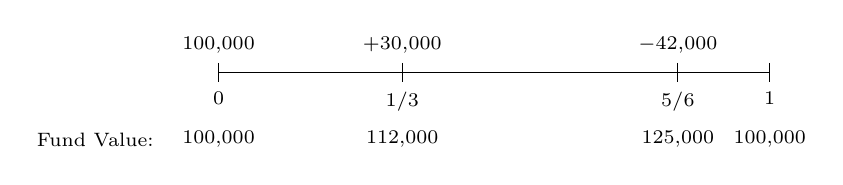
\begin{tikzpicture}
    \draw (0,0) -- (7,0);
    \foreach \x/\lab in {0/0, 2.333/{1/3}, 5.833/{5/6}, 7/1} {
      \draw (\x,0.12) -- (\x,-0.12);
      \node[below] at (\x,-0.12) {\scriptsize $\lab$};
    }
    \node[above] at (0,0.12) {\scriptsize 100,000};
    \node[above] at (2.333,0.12) {\scriptsize $+30{,}000$};
    \node[above] at (5.833,0.12) {\scriptsize $-42{,}000$};
    \node[anchor=east] at (-0.7,-0.85) {\scriptsize Fund Value:};
    \foreach \x/\v in {0/{100,000}, 2.333/{112,000}, 5.833/{125,000}, 7/{100,000}} {
      \node at (\x,-0.85) {\scriptsize \v};
    }
  \end{tikzpicture}%
}


\title{RISK 201: Rates of Return}

\begin{document}
\maketitle

%======================================================================
\section{Net present value}
%======================================================================

\begin{frame}{7.1 Net present value}

\underline{\textbf{Notation:}}

For $t = 0, 1, \ldots, n$,
\begin{itemize}
\item $A_t$: Amount \cin{received} at time $t$ from an investment
\item $B_t$: Amount \textcolor{red}{paid into} an investment at time $t$
\item $C_t = A_t - B_t$: \purple{net amount received} at time $t$ from an investment.
\end{itemize}

\bigskip
Usually, we have $C_0 < 0$ and $C_n > 0$.

\medskip
\begin{center}
\$ paid in \qquad\qquad \$ received
\end{center}

\end{frame}

\begin{frame}{Net present value (NPV)}

Let $P(i)$ denote the net present value of an investment, valued at rate $i$:
\[
P(i) = \sum_{t=0}^{n} C_t\, v^t
\]

\bigskip
The NPV is generally a \purple{decreasing} function of $i$.

\end{frame}

\begin{frame}{Example 7.1}

Consider the following series of cash flows:

\begin{center}
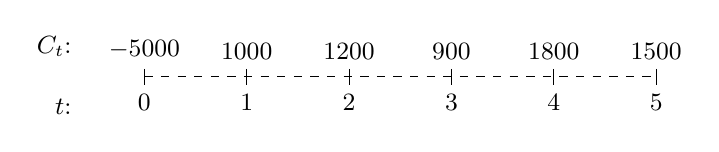
\begin{tikzpicture}
  \draw[dashed] (0,0) -- (6.5,0);
  \foreach \t/\c in {0/-5000, 1/1000, 2/1200, 3/900, 4/1800, 5/1500} {
    \draw (1.3*\t,0.1) -- (1.3*\t,-0.1);
    \node[above] at (1.3*\t,0.1) {\small $\c$};
    \node[below] at (1.3*\t,-0.1) {\small $\t$};
  }
  \node[anchor=east] at (-0.8,0.38) {\small $C_t$:};
  \node[anchor=east] at (-0.8,-0.38) {\small $t$:};
\end{tikzpicture}
\end{center}

\begin{columns}[c]
\column{0.38\textwidth}
\centering
\renewcommand{\arraystretch}{1.2}
\begin{tabular}{c|r}
$i$ & $P(i)$ \\
\hline
2\% & 1003.40 \\
5\% & 474.42 \\
10\% & $-262.18$ \\
\end{tabular}
\column{0.58\textwidth}
\centering
\begin{tikzpicture}[xscale=36, yscale=1.6]
  % vertical axis in thousands of dollars
  \draw[->] (0,0) -- (0.125,0) node[right] {\scriptsize $i$};
  \draw[->] (0,-0.35) -- (0,1.3) node[above] {\scriptsize $P(i)$};
  \foreach \y/\l in {-0.3/-300, 0.5/500, 1/1000} {
    \draw (-0.002,\y) -- (0.002,\y);
    \node[left] at (-0.002,\y) {\tiny $\l$};
  }
  \foreach \x/\l in {0.02/2\%, 0.05/5\%, 0.1/10\%} {
    \draw (\x,-0.025) -- (\x,0.025);
    \node[below] at (\x,-0.025) {\tiny \l};
  }
  \draw[thick, domain=0.015:0.11, samples=40, smooth]
    plot (\x, {(-5000 + 1000/(1+\x) + 1200/(1+\x)^2 + 900/(1+\x)^3 + 1800/(1+\x)^4 + 1500/(1+\x)^5)/1000});
\end{tikzpicture}
\end{columns}

\end{frame}

\begin{frame}{Discounted cash flow analysis}

\begin{itemize}
\item Every investor is assumed to have an \purple{investment preference rate ($i_p$)} which they would like to earn on their investments.
\item An investment is \cin{acceptable} if its NPV is \cin{positive} when valued at the investor's preference rate:
\[
P(i_p) = \sum_{t=0}^{n} C_t \frac{1}{(1+i_p)^t} > 0
\]
\item Normally, a higher \purple{$i_p$} makes an investment less desirable.
\end{itemize}

\end{frame}

\begin{frame}{Example 7.1, continued}

The cash flows are:

\begin{center}
\cfdiagram{6}{0/0, 1.2/1, 2.4/2, 3.6/3, 4.8/4, 6/5}%
  {0/\cout{$-5000$}, 1.2/\cin{1000}, 2.4/\cin{1200}, 3.6/\cin{900}, 4.8/\cin{1800}, 6/\cin{1500}}
\end{center}

If $i_p = 5\%$, $P(i_p) =$

\vfill
If $i_p = 10\%$, $P(i_p) =$

\vfill
\end{frame}

\begin{frame}{Example 7.2}

Consider the following stream of cash flows.

\begin{center}
\cfdiagram{6}{0/0, 3/1, 6/2}{0/\cout{$-1$}, 3/\cin{2.3}, 6/\cout{$-1.33$}}
\end{center}

If $i_p = 5\%$, $P(i_p) =$

\vfill
If $i_p = 15\%$, $P(i_p) =$

\vfill
\end{frame}

%======================================================================
\section{Internal rate of return}
%======================================================================

\begin{frame}{7.2 Internal rate of return}

The \purple{\textbf{internal rate of return (IRR)}} is the interest rate $i$ which satisfies
\[
P(i) = \sum_{t=0}^{n} C_t \frac{1}{(1+i)^t} = 0.
\]

An investor prefers a higher IRR; a borrower prefers a lower IRR.

\medskip
\begin{tabular}{rl}
IRR $> 0$ & the investment grows in value \\
$-1 <$ IRR $< 0$ & some of the original investment is lost \\
IRR $< -1$ & more than original investment is lost \\
\end{tabular}

\end{frame}

\begin{frame}{Example 7.1, continued}

\begin{center}
\cfdiagram{6}{0/0, 1.2/1, 2.4/2, 3.6/3, 4.8/4, 6/5}%
  {0/\cout{$-5000$}, 1.2/\cin{1000}, 2.4/\cin{1200}, 3.6/\cin{900}, 4.8/\cin{1800}, 6/\cin{1500}}
\end{center}

Confirm that the IRR is approximately 8.1\%.

\vfill
\end{frame}

\begin{frame}{Example 7.2, continued}

\begin{center}
\cfdiagram{6}{0/0, 3/1, 6/2}{0/\cout{$-1$}, 3/\cin{2.3}, 6/\cout{$-1.33$}}
\end{center}

\vfill
\end{frame}

\begin{frame}{Uniqueness of IRR}

\begin{itemize}
\item The IRR need not be positive, exist or be unique.
\item Descartes' rule of signs:
  \begin{itemize}
  \item The \purple{\textbf{maximum number of positive roots}} of an $n$th degree polynomial is equal to the \cin{\textbf{number of sign changes in the coefficients}}.
  \item If all the cash flows in one direction (i.e., $+$ or $-$) are made before the cash flows in the other direction, then the IRR is unique (because in this case, the number of sign changes $= 1$).
  \end{itemize}
\end{itemize}

\end{frame}

\begin{frame}{IRR method of capital budgeting}

\begin{enumerate}
\item Calculate the IRR of the investment
\item Compare this IRR to the interest preference rate ($i_p$) of the investor:
  \begin{itemize}
  \item if IRR $> i_p$, consider investment
  \item if IRR $< i_p$, reject investment
  \end{itemize}
\end{enumerate}

\end{frame}

\begin{frame}{IRR method of pricing}

\begin{enumerate}
\item Consider the investor's preference rate $i_p$.
\item Set the price of the investment so that the IRR is equal to $i_p$. This is equivalent to setting the NPV valued at $i_p$ to zero.
\end{enumerate}
\[
P(i_p) = \sum_{t=0}^{n} C_t \frac{1}{(1+i_p)^t} = 0
\]

\end{frame}

\begin{frame}{Example 7.3}

Consider an annuity that pays 155.82 at the end of each year for 10 years. If the investor's preference rate is 3\% per year, find the maximum price she is willing to pay for this annuity.

\begin{center}
\tenline{0/\cout{$X$}, 1.2/\cin{155.82}, 2.4/\cin{155.82}, 6/\cin{155.82}}
\end{center}

\vfill
\end{frame}

\begin{frame}{Borrowing to invest}

Suppose you are considering an investment opportunity but you don't actually have funds to invest $\rightarrow$ you can borrow money.
\begin{itemize}
\item The loan you receive should have the same term (length) as the investment.
\item You would only consider an investment if you could make a profit \blue{after taking into account the cost of the loan} (i.e., interest on the amount you borrowed).
\end{itemize}

\end{frame}

\begin{frame}{Example 7.4}

Consider the following investment:

\begin{center}
\tenline{0/\cout{$-1000$}, 1.2/\cin{155.82}, 2.4/\cin{155.82}, 3.6/\cin{155.82}, 4.8/$\ldots$, 6/\cin{155.82}}
\end{center}

Suppose you have to borrow the initial \$1000 needed to invest. If you can borrow at $i = 10\%$, should you go ahead?

\medskip
Q: Would the cash inflows from this investment cover the cost of borrowing at $i = 10\%$?

\end{frame}

\begin{frame}{Example 7.4, continued}

\begin{center}
\renewcommand{\arraystretch}{1.3}
\small
\begin{tabular}{crrrr}
\toprule
\textbf{Period} & \textbf{Payments} & \textbf{Interest} & \textbf{Principal} & \textbf{Loan balance} \\
\midrule
0 & & & & 1,000.00 \\
1 & 155.82 & 100.00 & 55.82 & 944.18 \\
2 & 155.82 & 94.42 & 61.40 & 882.78 \\
3 & 155.82 & 88.28 & 67.54 & 815.24 \\
\ldots & \ldots & \ldots & \ldots & \ldots \\
10 & 155.82 & 24.20 & 131.62 & 110.37 \\
\bottomrule
\end{tabular}
\end{center}

\end{frame}

\begin{frame}{Example 7.4, continued}

If the cost of borrowing is 10\%, borrowing to invest is \underline{not} profitable: cash inflows from investment are not enough to pay off the loan you took out to invest!

\medskip
In present value terms, at a rate of $i = 10\%$:
\[
\sum_{t=0}^{n} A_t \frac{1}{(1+i)^t} < \sum_{t=0}^{n} B_t \frac{1}{(1+i)^t}
\]
\[
P(0.1) = \sum_{t=0}^{n} A_t \frac{1}{(1.1)^t} - \sum_{t=0}^{n} B_t \frac{1}{(1.1)^t} = -42.55
\]

\end{frame}

\begin{frame}{Example 7.4, continued}

Would the cash inflows from this investment cover the cost of borrowing if you could borrow at 5\%?

\begin{center}
\renewcommand{\arraystretch}{1.3}
\small
\begin{tabular}{crrrr}
\toprule
\textbf{Period} & \textbf{Payments} & \textbf{Interest} & \textbf{Principal} & \textbf{Loan balance} \\
\midrule
0 & & & & 1,000.00 \\
1 & 155.82 & 50.00 & 105.82 & 894.18 \\
2 & 155.82 & 44.71 & 111.11 & 783.07 \\
3 & 155.82 & 39.15 & 116.67 & 666.40 \\
\ldots & \ldots & \ldots & \ldots & \ldots \\
10 & 155.82 & $-8.43$ & 164.16 & $-330.99$ \\
\bottomrule
\end{tabular}
\end{center}

\end{frame}

\begin{frame}{Example 7.4, continued}

If the cost of borrowing is 5\%, borrowing to invest is profitable: cash inflows from investment are more than enough to pay off the loan you took out!

\medskip
In present value terms, at a rate of $i = 5\%$:
\[
\sum_{t=0}^{n} A_t \frac{1}{(1+i)^t} > \sum_{t=0}^{n} B_t \frac{1}{(1+i)^t}
\]
\[
P(0.05) = \sum_{t=0}^{n} A_t \frac{1}{(1.05)^t} - \sum_{t=0}^{n} B_t \frac{1}{(1.05)^t} = 203.20
\]

\end{frame}

\begin{frame}{Example 7.4, continued}

What is the \purple{maximum loan rate} that would still allow you to invest without losing money?

\medskip
$\rightarrow$ Find $i$ such that
\[
P(i) = \sum_{t=0}^{n} A_t \frac{1}{(1+i)^t} - \sum_{t=0}^{n} B_t \frac{1}{(1+i)^t} = 0
\]

\vfill
\end{frame}

\begin{frame}{IRR, NPV, and the borrowing criterion}

By definition, the PV of cash inflows is exactly equal to the PV of cash outflows when valued at the IRR:
\[
\sum_{t=0}^{n} A_t \frac{1}{(1+\cin{IRR})^t} = \sum_{t=0}^{n} B_t \frac{1}{(1+\cin{IRR})^t}
\]

The IRR is the loan rate that would allow you to break even if you had to borrow the funds to invest.

\medskip
The net present value $P(i)$ is the PV of the profit you would make on your investment, after taking into account the cost of borrowing at rate $i$.

\end{frame}

\begin{frame}{Example 7.5}

Find the IRR of the following investments:

\medskip
(a)
\begin{center}
\tenline{0/\cout{$-1000$}, 6/\cin{2367.36}}
\end{center}

\vfill
(b)
\begin{center}
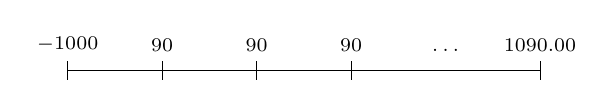
\begin{tikzpicture}
  \draw (0,0) -- (6,0);
  \foreach \x in {0, 1.2, 2.4, 3.6, 6} { \draw (\x,0.12) -- (\x,-0.12); }
  \foreach \x/\amt in {0/\cout{$-1000$}, 1.2/\cin{90}, 2.4/\cin{90}, 3.6/\cin{90}, 4.8/$\ldots$, 6/\cin{1090.00}} {
    \node[above] at (\x,0.12) {\scriptsize \amt};
  }
\end{tikzpicture}
\end{center}

\vfill
\end{frame}

\begin{frame}{Example 7.5, continued}

(c)
\begin{center}
\tenline{0/\cout{$-1000$}, 1.2/\cin{50}, 2.4/\cin{50}, 3.6/\cin{50}, 4.8/$\ldots$, 6/\cin{1657.72}}
\end{center}

\vfill
\end{frame}

\begin{frame}{Example 7.5, continued}

\begin{center}
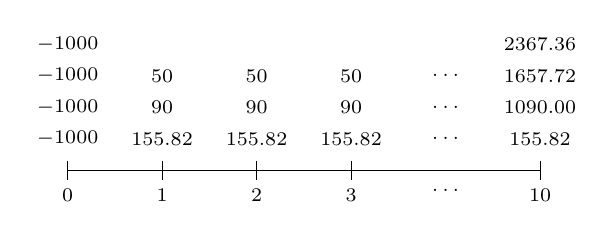
\begin{tikzpicture}
  \draw (0,0) -- (6,0);
  \foreach \x/\lab in {0/0, 1.2/1, 2.4/2, 3.6/3, 6/10} {
    \draw (\x,0.12) -- (\x,-0.12);
    \node[below] at (\x,-0.12) {\scriptsize $\lab$};
  }
  \node[below] at (4.8,-0.12) {\scriptsize $\ldots$};
  \foreach \row/\a/\b in {4/{}/{2367.36}, 3/{50}/{1657.72}, 2/{90}/{1090.00}, 1/{155.82}/{155.82}} {
    \node at (0,0.4*\row) {\scriptsize \cout{$-1000$}};
    \node at (1.2,0.4*\row) {\scriptsize \cin{\a}};
    \node at (2.4,0.4*\row) {\scriptsize \cin{\a}};
    \node at (3.6,0.4*\row) {\scriptsize \cin{\a}};
    \node at (6,0.4*\row) {\scriptsize \cin{\b}};
  }
  \foreach \row in {1,2,3} { \node at (4.8,0.4*\row) {\scriptsize $\ldots$}; }
\end{tikzpicture}
\end{center}

\vfill
\end{frame}

\begin{frame}{Taking into account reinvestment}

A \cin{reinvestment rate} is the rate at which a payment received from an original investment can be reinvested.

\medskip
When the proceeds of an investment are reinvested, the appropriate focal date for the valuation of cash inflows and outflows is at the \textbf{end} of the investment horizon.

\medskip
\begin{center}
$\Rightarrow$ compare AVs instead of PVs
\end{center}

\end{frame}

\begin{frame}{Yield rate}

A measure of the rate of return on an investment that takes reinvestment into account is the \textcolor{orange!90!red}{yield rate}.

\medskip
The yield rate \textcolor{orange!90!red}{$i$} satisfies
\[
\sum_{t=0}^{n} A_t\,(1+\cin{j})^{n-t} = \sum_{t=0}^{n} B_t\,(1+\textcolor{orange!90!red}{i})^{n-t}
\]
where \cin{$j$} is the reinvestment rate.

\end{frame}

\begin{frame}{Yield rate and the borrowing criterion}

You can think of the yield rate as the loan rate \textcolor{orange!90!red}{$i$} that would allow you to break even if you had to borrow the funds to invest, and you waited until the end of the horizon to repay the loan, while accumulating cash inflows in a fund earning \cin{$j$}:
\[
\sum_{t=0}^{n} A_t\,(1+\cin{j})^{n-t} = \sum_{t=0}^{n} B_t\,(1+\textcolor{orange!90!red}{i})^{n-t}
\]

\end{frame}

\begin{frame}{Example 7.6}

Find the yield rate on the following investment if

\medskip
(a) the reinvestment rate is 5\%.

\begin{center}
\tenline{0/\cout{$-1000$}, 1.2/\cin{155.82}, 2.4/\cin{155.82}, 3.6/\cin{155.82}, 4.8/$\ldots$, 6/\cin{155.82}}
\end{center}

\vfill
\end{frame}

\begin{frame}{Example 7.6, continued}

(b) the reinvestment rate is 7\%.

\begin{center}
\tenline{0/\cout{$-1000$}, 1.2/\cin{155.82}, 2.4/\cin{155.82}, 3.6/\cin{155.82}, 4.8/$\ldots$, 6/\cin{155.82}}
\end{center}

\vfill
\end{frame}

\begin{frame}{Example 7.6, continued}

(c) the reinvestment rate is 9\%.

\begin{center}
\tenline{0/\cout{$-1000$}, 1.2/\cin{155.82}, 2.4/\cin{155.82}, 3.6/\cin{155.82}, 4.8/$\ldots$, 6/\cin{155.82}}
\end{center}

\vfill
\end{frame}

%======================================================================
\section{Dollar-weighted rates}
%======================================================================

\begin{frame}{7.3 Dollar-weighted rates}

\underline{\textbf{Notation:}}
\begin{itemize}
\item $A$: Amount in fund at $t = 0$
\item $B$: Amount in fund at $t = 1$
\item $I$: Interest earned in the year
\item $n_t$: New principal added at time $t$, $(0 \le t \le 1)$
\item $n = \sum n_t$: total new principal added during year
\item $w_t$: Principal withdrawn at time $t$, $(0 \le t \le 1)$
\item $w = \sum w_t$: total withdrawals during year
\end{itemize}
\[
B = A + n - w + I
\]

\end{frame}

\begin{frame}{Equation of value}

\begin{center}
\cfdiagram{7}{0/0, 7/1}{0/$A$}
\end{center}

If we assume \textcolor{red}{compound interest} during the year:
\[
B = A(1+i) + \sum n_t \textcolor{red}{(1+i)^{1-t}} - \sum w_t \textcolor{red}{(1+i)^{1-t}}
\]

We know that the interest rate $i$ that satisfies this equation is the \textcolor{red}{IRR}. But solving this is cumbersome.

\end{frame}

\begin{frame}{A simple approximation}

If we assume \cin{simple interest} during the year, the equation of value at $t = 1$ becomes
\[
B = A(1+i) + \sum n_t \cin{\bigl(1 + i(1-t)\bigr)} - \sum w_t \cin{\bigl(1 + i(1-t)\bigr)}
\]
\[
B = A + n - w + iA + \sum n_t\, i(1-t) - \sum w_t\, i(1-t)
\]

\end{frame}

\begin{frame}{Dollar-weighted rate of interest}

The \textbf{dollar-weighted rate of interest} is an approximation to the actual rate of interest earned, based on the simple interest assumption:
\[
i \approx \frac{I}{A + \sum n_t(1-t) - \sum w_t(1-t)}
\]

\medskip
This is usually a good approximation, especially if the $n_t$ and $w_t$ are small compared to $A$.

\end{frame}

\begin{frame}{Example 7.7}

Consider the following pension fund:

\begin{center}
\pensionfund
\end{center}

Calculate the dollar-weighted rate of interest.

\vfill
\end{frame}

\begin{frame}{A further simplification}

If we assume that the cash flows $n$ and $w$ occur uniformly throughout the year (midyear on average)
\[
i \approx \frac{I}{A + 0.5n - 0.5w}
\]

\medskip
This is widely used in practice, but provides a poor approximation if the timing of the cash flows differs significantly from the assumption.

\end{frame}

\begin{frame}{Example 7.7, continued}

Consider the following pension fund:

\begin{center}
\pensionfund
\end{center}

Recalculate the dollar-weighted rate of interest using the midyear assumption.

\vfill
\end{frame}

%======================================================================
\section{Time-weighted rates}
%======================================================================

\begin{frame}{7.4 Time-weighted rates}

\begin{enumerate}
\item Divide the period under consideration into $m$ successive subintervals each time a deposit or withdrawal is made.
\item Denote subinterval $k$ as $[t_{k-1}, t_k]$
\item Calculate the fund balance $B_t$ at the end of each subinterval, just before each cash flow
\item Calculate the rate of return during subinterval $k$ as
\[
1 + j_k = \frac{B_{t_k}}{B_{t_{k-1}} + n_{t_{k-1}} - w_{t_{k-1}}}
\]
\end{enumerate}

\end{frame}

\begin{frame}{Time-weighted rates}

\begin{enumerate}
\setcounter{enumi}{4}
\item Then the time-weighted rate of interest, $i$, earned over the entire year is calculated as
\[
1 + i = \prod_{k=1}^{m} (1 + j_k)
\]
\end{enumerate}

\medskip
Note: Time-weighted rates are \underline{not} consistent with compound interest, but they are usually better indicators of the performance (or effectiveness) of the investment manager.

\end{frame}

\begin{frame}{Example 7.7, continued}

Consider the following pension fund:

\begin{center}
\pensionfund
\end{center}

Calculate the time-weighted rate of interest for the fund.

\vfill
\end{frame}

%======================================================================
\section{Other securities}
%======================================================================

\begin{frame}{7.5 Other securities}

Debt versus equity in the corporate structure:
\begin{itemize}
\item Debt holders are called creditors; they always get paid unless the borrower defaults on the loan
  \begin{itemize}
  \item Secured creditors (have lien on assets)
  \item Unsecured creditors (no lien)
  \end{itemize}
\item Equity holders (aka shareholders) are entitled to residual profits, after everyone else is paid
  \begin{itemize}
  \item Periodic disbursements of profits to shareholders are called dividends
  \end{itemize}
\end{itemize}

\end{frame}

\begin{frame}{Different types of securities}

\begin{itemize}
\item Equity securities:
  \begin{itemize}
  \item Preferred stock: fixed dividends, paid before common stock dividends
  \item Common stock: dividend varies with profits
  \end{itemize}
\item Debt securities
  \begin{itemize}
  \item Bonds (Chapter 6)
  \end{itemize}
\end{itemize}

\end{frame}

\begin{frame}{Dividend discount model}

\begin{itemize}
\item Notation
  \begin{itemize}
  \item $D$: amount of next dividend payment
  \item $i$: investor's desired rate of return (yield)
  \item $g$: growth rate of the dividend
  \item $P$: price of the stock
  \end{itemize}
\item Stock price according to dividend discount model
\[
P = \frac{D}{1+i} + \frac{D(1+g)}{(1+i)^2} + \frac{D(1+g)^2}{(1+i)^3} + \cdots = \frac{D}{i-g}
\]
\end{itemize}

\end{frame}

\begin{frame}{Example 7.8}

The earnings of a corporation are expected to increase 3\% per year. The current earnings on a common stock are \$5 per share. The corporation pays 60\% of its earnings as dividends. Find the price per share that will yield 4.5\%.

\vfill
\end{frame}

\end{document}
